../cictikz/src/cictikz/data/tex/cictikz_preamble.tex

% The four logic values fall out of which network is on: Z when neither,
% X when both, and the two digital values in between.

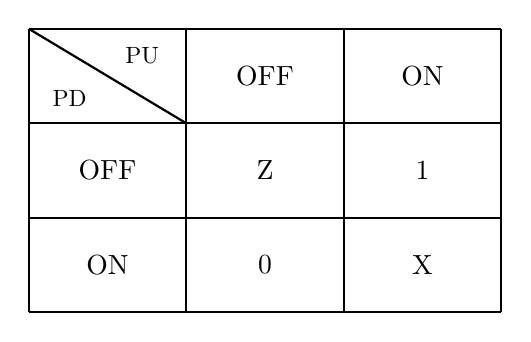
\begin{tikzpicture}[thick]

  \def\cw{2.0}   % column width
  \def\rh{1.2}   % row height

  % grid
  \draw ({0},{-2*\rh}) -- ({0},\rh);
  \draw ({\cw},{-2*\rh}) -- ({\cw},\rh);
  \draw ({2*\cw},{-2*\rh}) -- ({2*\cw},\rh);
  \draw ({3*\cw},{-2*\rh}) -- ({3*\cw},\rh);
  \draw (0,\rh) -- ({3*\cw},\rh);
  \draw (0,0) -- ({3*\cw},0);
  \draw ({0},{-\rh}) -- ({3*\cw},{-\rh});
  \draw ({0},{-2*\rh}) -- ({3*\cw},{-2*\rh});

  % header cell with the diagonal
  \draw (0,\rh) -- (\cw,0);
  \node[scale=0.85] at ({0.72*\cw},{0.72*\rh}) {PU};
  \node[scale=0.85] at ({0.26*\cw},{0.26*\rh}) {PD};

  % headers
  \node at ({1.5*\cw},{0.5*\rh}) {OFF};
  \node at ({2.5*\cw},{0.5*\rh}) {ON};
  \node at ({0.5*\cw},{-0.5*\rh}) {OFF};
  \node at ({0.5*\cw},{-1.5*\rh}) {ON};

  % values
  \node at ({1.5*\cw},{-0.5*\rh}) {Z};
  \node at ({2.5*\cw},{-0.5*\rh}) {1};
  \node at ({1.5*\cw},{-1.5*\rh}) {0};
  \node at ({2.5*\cw},{-1.5*\rh}) {X};

\end{tikzpicture}
\end{document}
